% !TEX program = xelatex

\documentclass[12pt,a4paper]{article}
\usepackage[UTF8]{ctex}
\usepackage{float}
\usepackage{amsmath}
\usepackage{amsfonts}
\usepackage{enumerate}
\usepackage{booktabs}
\usepackage{graphicx}
\usepackage{longtable}
\usepackage{subfigure}

\usepackage{url}
\usepackage{multirow}

% for plotting 
\usepackage{caption}
\usepackage{pgfplots}

% for pseudo code 
\usepackage{algorithm}
\usepackage[noend]{algpseudocode}

% for reference 
\usepackage{hyperref}
\usepackage{cleveref}

% for code 
\usepackage{listings}
\usepackage{xcolor}
\usepackage{fontspec}
\definecolor{darkgreen}{rgb}{0,0.6,0}
\newfontfamily\consolas{Consolas}

\lstset {
    basicstyle=\footnotesize\consolas, % basic font setting
    breaklines=true, 
    frame=single,     % {single, shadowbox, bottomline}
    keywordstyle=\color{blue}, 
    commentstyle=\color{darkgreen},
    stringstyle=\color{red},
    showstringspaces=false,
    % backgroundcolor=\color{black!5}, % set backgroundcolor
    numbers=left, 
    numberstyle=\ttfamily,
}

% Microsoft Word A4 paper default layout 
\usepackage[a4paper, left=3.18cm, right=3.18cm, top=2.54cm, bottom=2.54cm]{geometry}

% \captionsetup[figure]{labelfont={bf}, name={Figure}}
% \captionsetup[table]{labelfont={bf}, name={Table}}

\crefname{equation}{方程}{方程}
\Crefname{equation}{方程}{方程}
\crefname{table}{表}{表}
\Crefname{table}{表}{表}
\crefname{figure}{图}{图}
\Crefname{figure}{图}{图}

\title{数学实验:第五次作业}
\author{计算机系 \quad 计73 \quad 2017011620 \quad 李家昊}
\date{\today}

% 实验报告格式的基本要求

% 系别、班级、学号、姓名

% 1 实验目的
% 2 题目
%   2.1 计算题:题号,算法设计(包括计算公式),程序,计算结果(计算机输出),结果分析,结论。
%   2.2 应用题:题号,问题分析,模型假设,模型建立,算法设计(包括计算公式),程序,计算结果(计算机输出),结果的数学分析,结果的实际意义,结论。
% 3 收获与建议

% Calc
% \subsubsection{算法设计}
% \subsubsection{Matlab程序}
% \subsubsection{计算结果}
% \subsubsection{结果分析}
% \subsubsection{结论}

% App
% \subsubsection{问题分析}
% \subsubsection{模型假设}
% \subsubsection{模型建立}
% \subsubsection{算法设计}
% \subsubsection{Matlab程序}
% \subsubsection{计算结果}
% \subsubsection{结果的数学分析}
% \subsubsection{结果的实际意义}
% \subsubsection{结论}

\begin{document}

\maketitle

\section{实验目的}

\begin{itemize}
    \item 掌握MATLAB优化工具箱的基本用法,对不同算法进行初步分析、比较。
    \item 练习用无约束优化方法建立和求解实际问题的模型(包括非线性最小二乘拟合)。
    \item 掌握用MATLAB优化工具箱和LINGO解线性规划的方法。
    \item 练习建立实际问题的线性规划模型。
\end{itemize}

\section{问题求解}

\subsection{Chap7-Ex5 原子位置(应用题)}

\subsubsection{问题分析}

题目给定某个分子的原子个数,以及某些原子对之间的距离,需要确定每个原子的相对位置。对于该问题,可以求出一组最优的原子相对位置,使得原子之间的距离尽可能接近给定的距离,即两者之间的误差尽可能小,这就构成了一个无约束优化问题。

\subsubsection{模型假设}

为了简化实际问题,模型基于以下假设,
\begin{enumerate}
    \item 该分子为平面分子,所有原子处于同一平面上。
    \item 该分子的结构稳定,所有原子之间的距离固定不变。
    \item 给定的原子对距离是原子位置的唯一约束。
\end{enumerate}

\subsubsection{模型建立}

设原子个数为$n$,不失一般性,不妨以第$n$个原子作为参考系,即第$n$个原子的坐标为$(0,0)$,设第$i$个原子的坐标为$(x_i, y_i)$($i = 1,2,\cdots,n-1$),题目给定的原子对距离约束$(i, j, d_{ij})$构成集合$\mathcal{D}$,其中$d_{ij}$表示第$i$个原子与第$j$个原子之间的距离,为了满足给定约束,原子距离需要尽可能满足下式,
\begin{equation}\label{eq:ex5_equal}
    \sqrt{(x_i-x_j)^2 + (y_i-y_j)^2} = d_{ij}, \quad (i,j,d_{ij}) \in \mathcal{D}
\end{equation}
在本题中,\Cref{eq:ex5_equal}确定了52个方程,但只包含48个变量,属于超定方程组,一般来说没有精确解,因此只能求出最小二乘意义下的最优解,其优化目标为,
\begin{equation}\label{eq:ex5_model}
    \min z = \sum_{(i,j,d_{ij}) \in \mathcal{D}} \left|\sqrt{(x_i-x_j)^2 + (y_i-y_j)^2} - d_{ij}\right|^2
\end{equation}
\Cref{eq:ex5_model}即为本题的模型。

\subsubsection{算法设计}

\Cref{eq:ex5_model}是一个无约束优化问题,可采用最速下降法和拟牛顿法求解,对应的命令为\texttt{fminunc},同时它也是一个非线性最小二乘问题,也可采用LM方法和置信域方法求解,对应的命令为\texttt{lsqnonlin}。

\subsubsection{Matlab程序}

请参见附录\ref{sec:ex5_code}。

\subsubsection{计算结果}

\begin{table}[t]
    \centering
    \caption{五种方法求解得出的最优值,所需迭代次数及目标函数调用次数}
    \label{tab:ex5_result}
    \begin{tabular}{c|ccc}
        \toprule
        Method & $z_{\min}$& Iterations & Func Count\tabularnewline
        \midrule
        SteepDesc & 5.7759 & 548 & 53802\tabularnewline
        BFGS & 0.0246 & 196 & 10143\tabularnewline
        DFP & 0.0471 & 10001 & 491225\tabularnewline
        LM & 0.0575 & 60 & 3023\tabularnewline
        TRM & 0.0602 & 161 & 7938\tabularnewline
        \bottomrule
    \end{tabular}
\end{table}

将48个变量的初值置为全零,分别通过最速下降法(SteepDesc),拟牛顿法的BFGS公式,拟牛顿法的DFP公式,LM方法,以及置信域(TRM)方法计算原子的位置,求解结果如\Cref{tab:ex5_result}所示,表中列出了五种方法求出的最优值,所用的迭代次数,以及目标函数的调用次数,其中DFP公式因迭代次数超过最大值而提前终止。

为了进一步探索模型的稳定性,这里在区间$(-1, 1)$内取48个独立均匀分布的随机数,作为变量的初值,用BFGS公式进行求解,结果如\Cref{fig:ex5_zmin}所示。

在上述的初值条件探索过程中,取出最优值最小的一组解,作为原子相对位置的最终结果,如\Cref{fig:ex5_coords}所示,其最优值为0.0070,原子的相对坐标如\Cref{tab:ex5_coords}所示,其中只列出了前24个原子的坐标,第25个原子的坐标为$(0,0)$。

\begin{figure}[t]
    \centering
    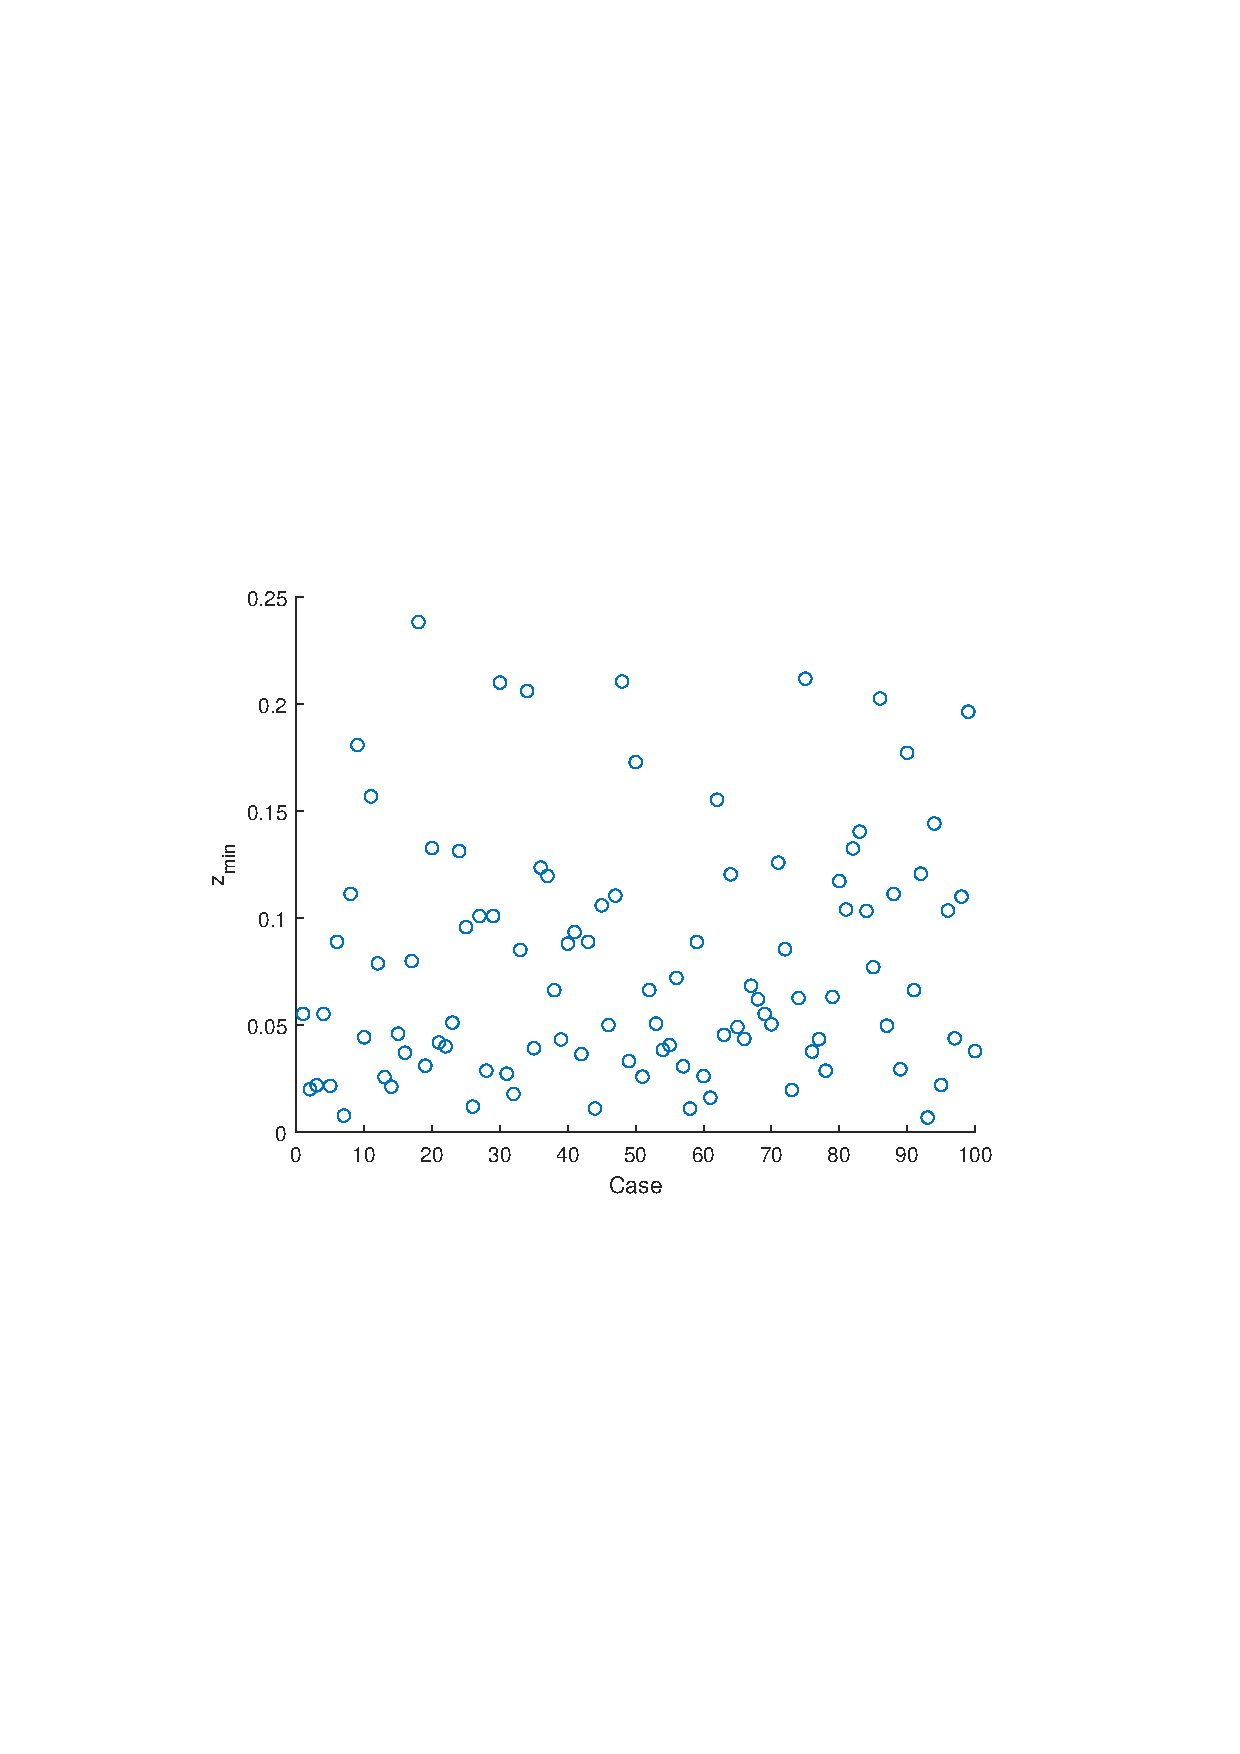
\includegraphics[width=0.8\textwidth,trim={3.09cm 9.295cm 3.09cm 9.295cm},clip]{fig/ex5_zmin.pdf}
    \caption{多次随机选取初始值,采用BFGS公式求解得到的最优值}
    \label{fig:ex5_zmin}
\end{figure}

\begin{figure}[t]
    \centering
    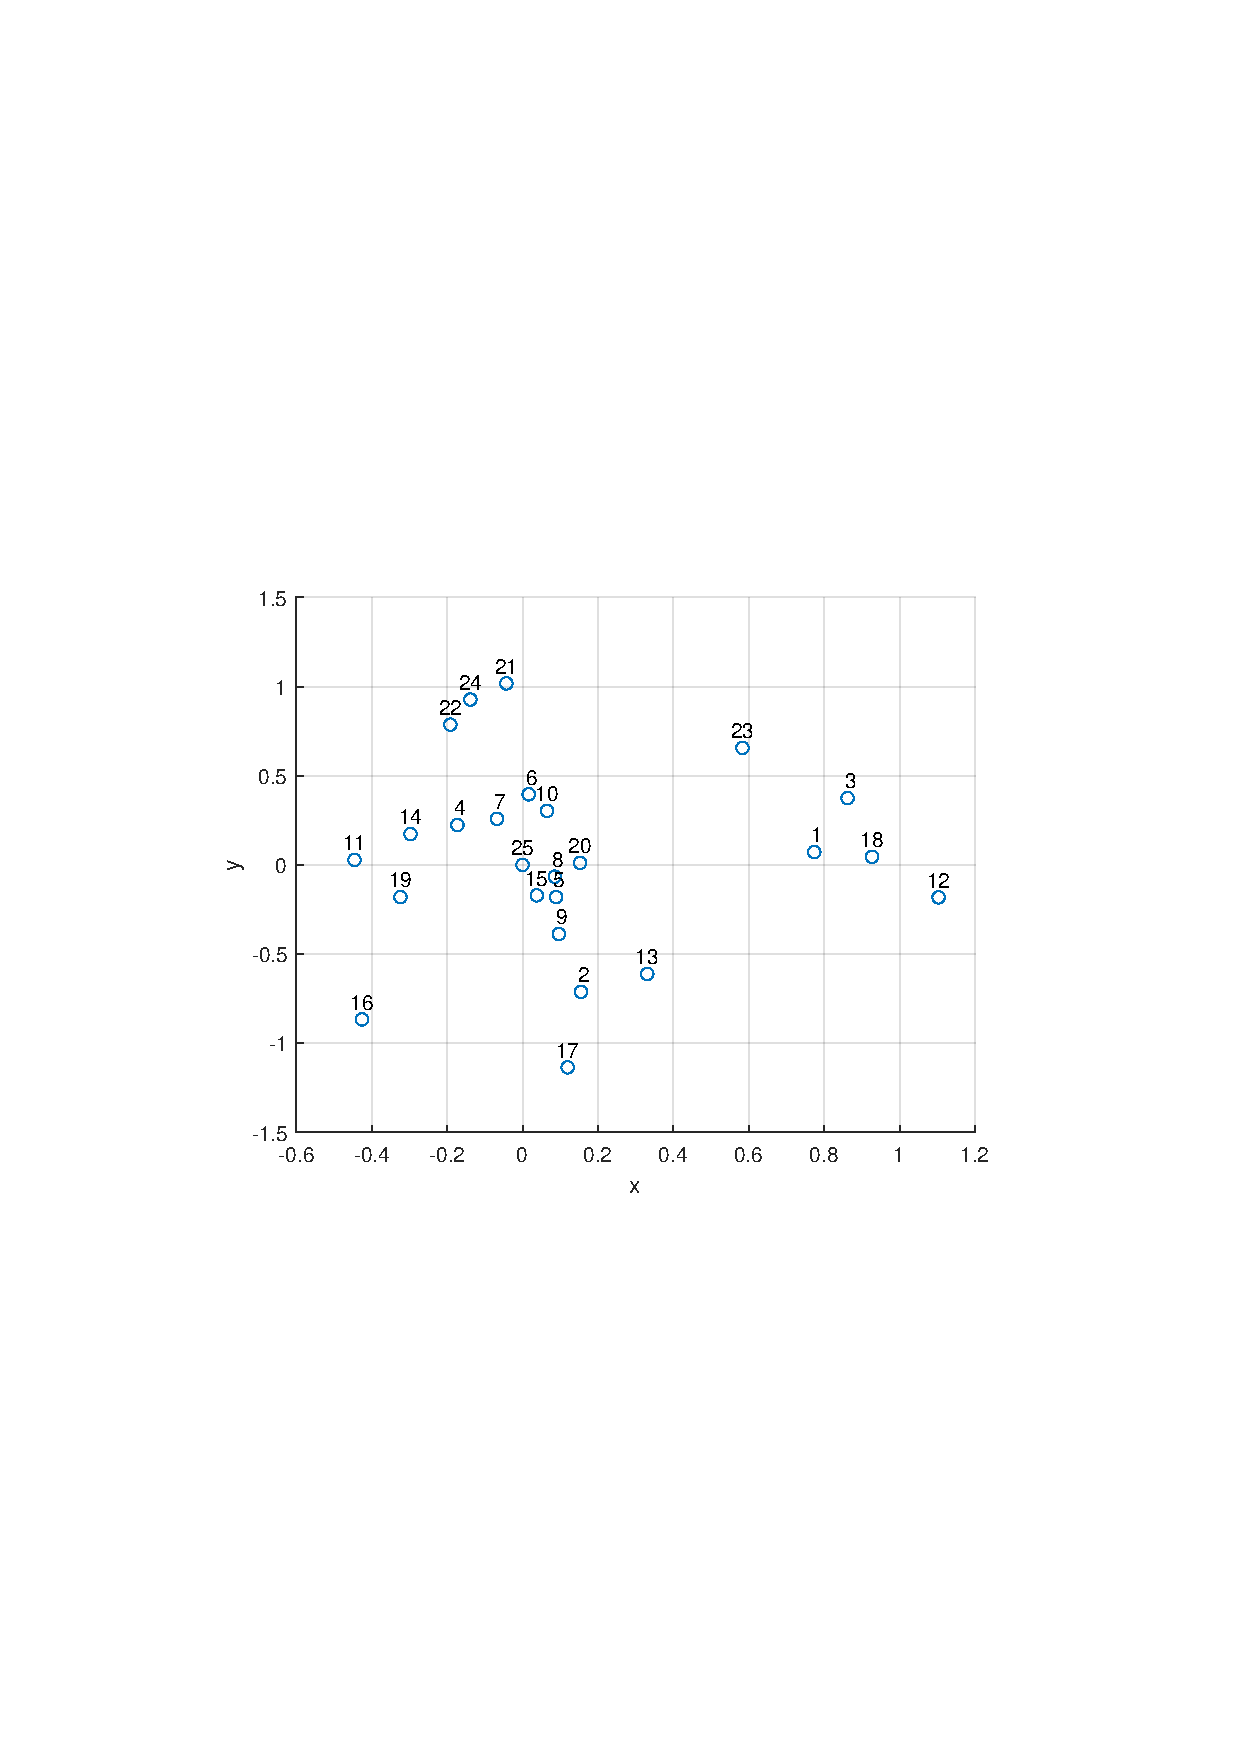
\includegraphics[width=0.75\textwidth,trim={3.09cm 9.295cm 3.09cm 9.295cm},clip]{fig/ex5_coords.pdf}
    \caption{相对于第25个原子,第1-24个原子的位置}
    \label{fig:ex5_coords}
\end{figure}

\begin{table}[h]
    \centering 
    \caption{相对于第25个原子,第1-24个原子位置的数值结果}
    \label{tab:ex5_coords}
    \begin{tabular}{ccc|ccc|ccc}
        \toprule
        No. & \(x\) & \(y\) & No. & \(x\) & \(y\) & No. & \(x\) &
        \(y\)\tabularnewline
        \midrule
        1 & 0.7735 & 0.0720 & 9 & 0.0964 & -0.3875 & 17 & 0.1195 &
        -1.1353\tabularnewline
        2 & 0.1549 & -0.7119 & 10 & 0.0648 & 0.3029 & 18 & 0.9269 &
        0.0457\tabularnewline
        3 & 0.8619 & 0.3747 & 11 & -0.4456 & 0.0281 & 19 & -0.3240 &
        -0.1804\tabularnewline
        4 & -0.1729 & 0.2237 & 12 & 1.1031 & -0.1822 & 20 & 0.1525 &
        0.0113\tabularnewline
        5 & 0.0889 & -0.1802 & 13 & 0.3306 & -0.6111 & 21 & -0.0429 &
        1.0177\tabularnewline
        6 & 0.0164 & 0.3961 & 14 & -0.2973 & 0.1729 & 22 & -0.1914 &
        0.7867\tabularnewline
        7 & -0.0681 & 0.2586 & 15 & 0.0377 & -0.1707 & 23 & 0.5830 &
        0.6564\tabularnewline
        8 & 0.0855 & -0.0659 & 16 & -0.4258 & -0.8661 & 24 & -0.1383 &
        0.9274\tabularnewline
        \bottomrule
    \end{tabular}
\end{table}

\subsubsection{结果的数学分析}

\paragraph{不同方法的对比} 由\Cref{tab:ex5_result}可以看出,在全零初值条件下,最速下降法的结果最差,在本题条件下并不收敛,拟牛顿法的BFGS公式的精度最高,迭代次数较少,DFP公式精度较高,但收敛较慢,迭代次数较多,LM算法的迭代次数最少,精确度较高,TRM方法相比LM算法精度较低,收敛较慢。在效率和精度的综合考虑下,对于该非线性无约束优化问题,BFGS的求解性能最佳,因此这里采用BFGS公式来计算原子相对位置的最终结果。

\paragraph{稳定性分析} 由\Cref{fig:ex5_zmin}观察到,最终结果对初值十分敏感,在100组随机选取的初值条件下,求解得到的最优值差异悬殊,最大超过0.2,最小低于0.01,跨越了一个数量级,由此确定的最终原子位置也千差万别。其原因是在不同初值条件下,算法收敛到了不同的局部极小值,而不能收敛到全局最小值。这种情况是人们不愿意看到的,但在实际应用中却普遍存在,例如在深度学习中,模型权重的不同初始值通常会带来不同的收敛结果。为了跳出局部极小值,人们提出了多种方法,例如梯度下降中的动量项,Adam优化器中学习率的动态调整等等。

\paragraph{误差分析} 最终的原子位置结果如\Cref{fig:ex5_coords}和\Cref{tab:ex5_coords}所示,对应的最优值为0.0070,这同时也是原子对距离误差的平方和,误差相对偏高。

\subsubsection{结果的实际意义}

在最终结果下,原子对距离误差的平方和为0.0070,有一定的实际参考价值,但不能确定是否还有更优的解,因此该分子的结构还需进一步由实验确定。实际上,该分子有可能是立体分子,在这种情况下,则需要更多的原子对距离约束,才能确定原子的相对位置。

\subsubsection{结论}

原子相对位置如\Cref{fig:ex5_coords}和\Cref{tab:ex5_coords}所示。

\subsection{Chap7-Ex8 给药方案(计算题)}

\subsubsection{算法设计}

\paragraph{模型} 由题意,这里采用一室模型,将整个机体看作一个中心室,口服给药过程可简化为在药物进入中心室之前有一个吸收室。记中心室和吸收室的容积分别为$V$和$V_1$,而$t$时刻的血药浓度分别为$c(t)$和$c_1(t)$,中心室的排除速率为$k$,吸收速率为$k_1$,设$t=0$时刻口服剂量为$d$的药物,则吸收室的血药浓度$c_1(t)$的微分方程为,
\begin{equation}
    \frac{dc_1}{dt} = -k_1 c_1, \quad c_1(0) = \frac{d}{V_1}
\end{equation}
中心室血药浓度$c(t)$的变化率由两部分组成:与$c$成正比的排除,与$c_1$成正比的吸收。考虑到中心室和吸收室的容积分别为$V$和$V_1$,得到$c(t)$的微分方程为,
\begin{equation}
    \frac{dc}{dt} = -kc + \frac{V_1}{V}k_1 c_1, \quad c(0) = 0
\end{equation}
由以上两个方程可解出中心室血药浓度为,
\begin{equation}
    c(t) = \frac{d}{V}\frac{k_1}{k_1 - k}(e^{-kt} - e^{-k_1 t})
\end{equation}
在制定给药方案时,需要根据实验数据确定$k, k_1, b$三个参数,其中$b=d/V$。

记给定的实验数据为$\{(t_i, c_i)\}_{i=1}^n$,则确定了$n$个方程,在本题条件下$n>3$,因此方程组为超定方程,只能在最小二乘意义下求得最优解,其优化目标为,
\begin{equation}\label{eq:ex8_model}
    \min z = \sum_{i=1}^n\left|c(t_i) - c_i\right|^2
\end{equation}
\Cref{eq:ex8_model}即为本题的模型。

\paragraph{算法} 考虑到比例系数$k, k_1$一般非负,口服剂量$d$和中心室容积$V$必然非负,即题目暗含了$k,k_1, b \ge 0$这个约束,因此\Cref{eq:ex8_model}是一个有约束优化问题,但是在实践中可以用无约束优化方法求解,只需确保最终答案满足非负约束即可,因此可以采用最速下降法,拟牛顿法的BFGS公式和DFP公式求解,对应的命令是\texttt{fminunc},同时,它也是一个最小二乘拟合问题,因此也可以用LM和置信域方法求解,对应的命令是\texttt{lsqcurvefit},它与\texttt{lsqnonlin}命令所用算法相同,但调用接口更加友好。特别的,采用置信域方法求解时,规定$k,k_1,b$的最小值均为0。

\subsubsection{Matlab程序}

请参见附录\Cref{sec:ex8_code}。

\subsubsection{计算结果}

在初值为$k=0.1, k_1=1, b=10$时,分别用最速下降法(SteepDesc),拟牛顿法的BFGS和DFP公式,LM方法,置信域方法(TRM)求解所得的$k,k_1,b$结果如\Cref{tab:ex8_result}所示,其中最速下降法由于不收敛导致程序崩溃退出,求解失败。将置信域方法的求解结果作为最终结果,其对应的$c(t)$拟合曲线如\Cref{fig:ex8_fit}所示。

\begin{table}
    \centering
    \caption{五种方法的$k,k_1,b$求解结果,最优值,所需迭代次数,目标函数调用次数}
    \label{tab:ex8_result}
    \begin{tabular}{c|ccc|ccc}
        \toprule
        Method & \(k\) & \(k_1\) & \(b\) & $z_{\min}$& Iterations &
        Func Count\tabularnewline
        \midrule
        SteepDesc & / & / & / & / & / & /\tabularnewline
        BFGS & 0.2803 & 3.6212 & 46.8275 & 34.2317 & 43 & 243\tabularnewline
        DFP & 0.3228 & 4.4308 & 45.4464 & 103.6406 & 10001 &
        40223\tabularnewline
        LM & 0.2803 & 3.6212 & 46.8275 & 34.2317 & 7 & 35\tabularnewline
        TRM & 0.2803 & 3.6212 & 46.8275 & 34.2317 & 7 & 32\tabularnewline
        \bottomrule
    \end{tabular}
\end{table}

\begin{figure}[t]
    \centering
    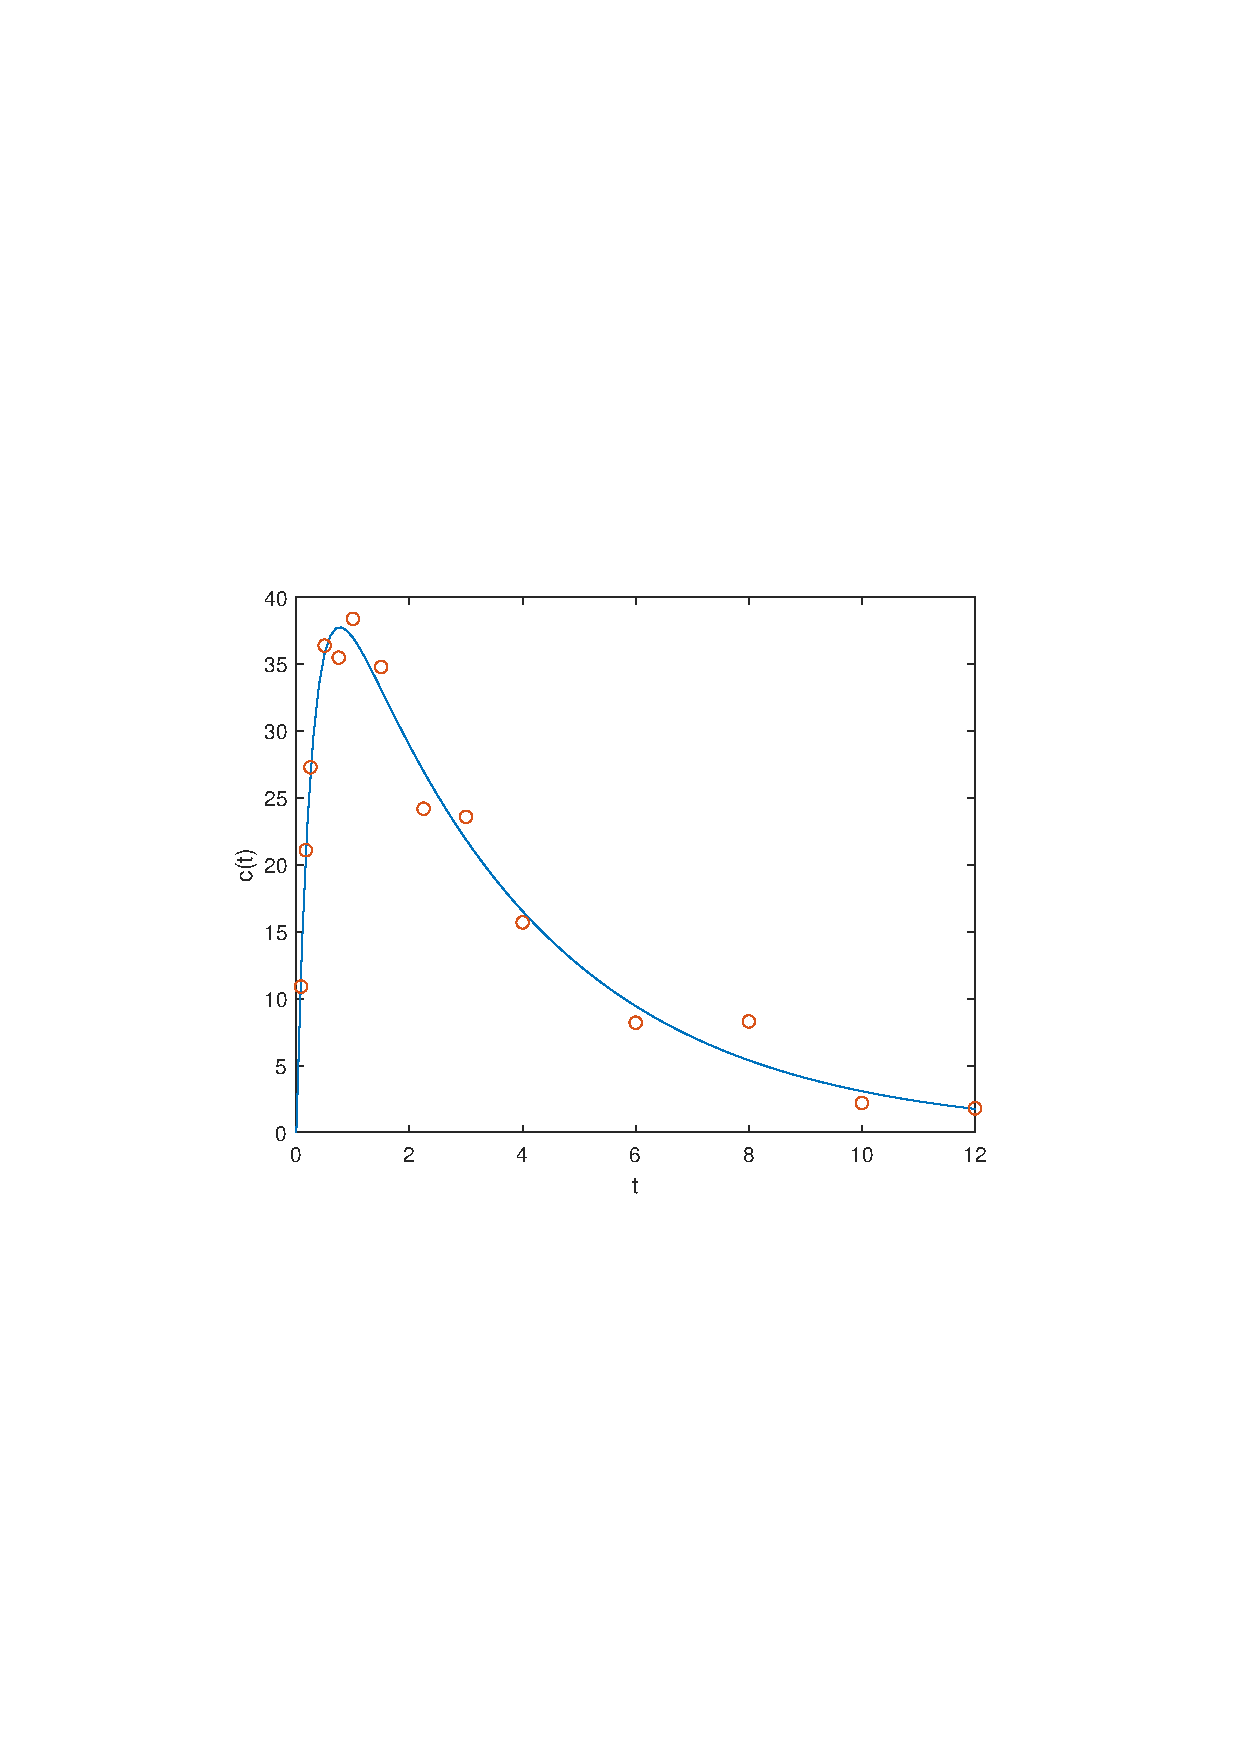
\includegraphics[width=0.8\textwidth,trim={3.09cm 9.295cm 3.09cm 9.295cm},clip]{fig/ex8_fit.pdf}
    \caption{原始实验数据以及置信域方法求得的拟合曲线}
    \label{fig:ex8_fit}
\end{figure}

\begin{figure}[t]
    \centering
    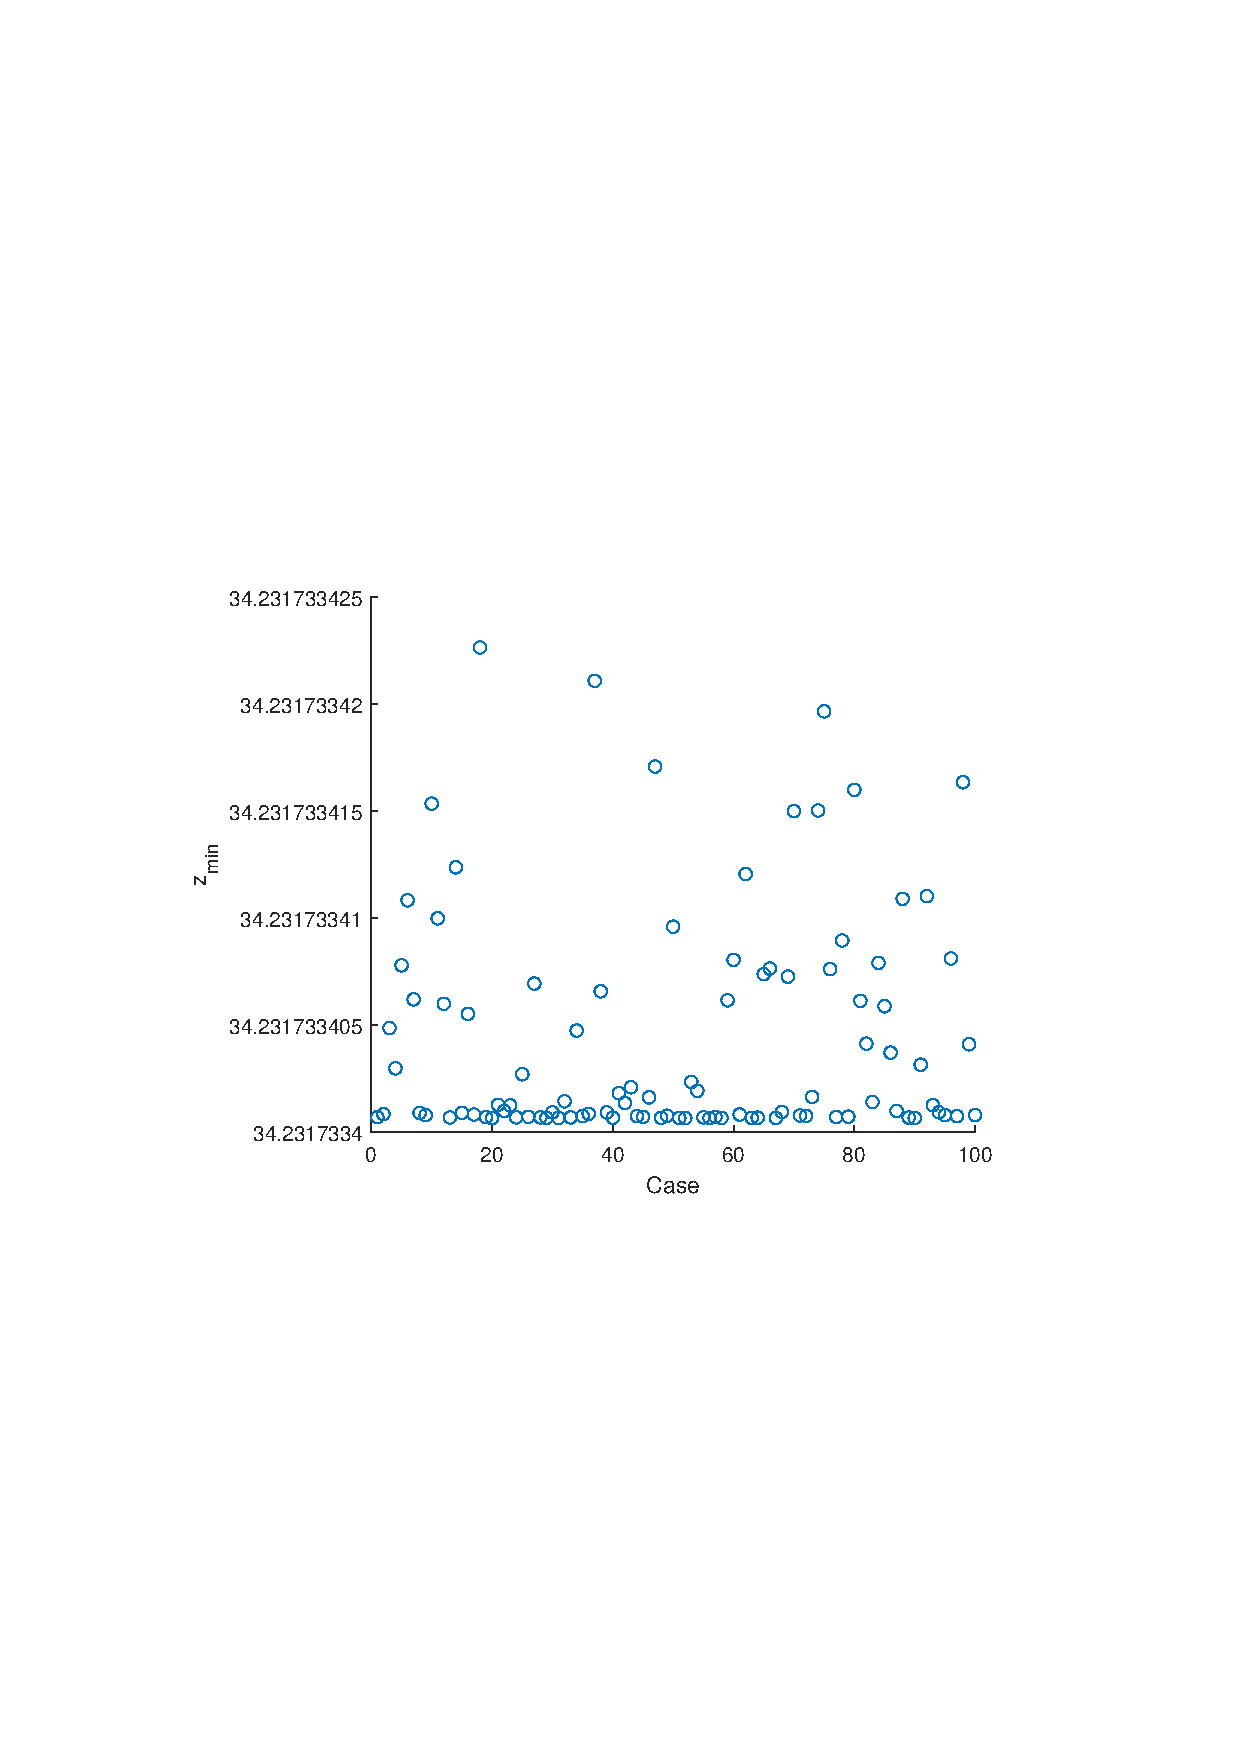
\includegraphics[width=0.8\textwidth,trim={3.09cm 9.295cm 3.09cm 9.295cm},clip]{fig/ex8_init.pdf}
    \caption{多次随机选取初始值,采用置信域方法求解得到的最优值}
    \label{fig:ex8_init}
\end{figure}

为了进一步分析模型的稳定性,这里同样随机选取100组初值,令$k,k_1$在$(0, 10)$区间内独立均匀地随机选取,令$b$在$(0,100)$区间内均匀地随机选取,求解得到的最优值如\Cref{fig:ex8_init}所示,经过计算,这100个最优值的标准差为$4.6372\times 10^{-9}$,$k,k_1,b$的标准差分别为$4.8745\times 10^{-7}$,$4.3622\times 10^{-6}$,$3.3112\times 10^{-5}$。

\subsubsection{结果分析}

\Cref{tab:ex8_result}又一次验证了,在五种方法中,最速下降法的效果最差,在本题条件下根本不收敛,拟牛顿法的BFGS公式和DFP公式的精度和效率一般,LM方法和置信域方法的精度和效率最优。

在给定范围内多次随机选取初值,采用置信域方法求解的结果差异极小,说明模型十分稳定,对初值不敏感,而且有理由相信,\Cref{tab:ex8_result}中的结果已经是全局最优值,因此具有实际应用价值,可作为制定给药方案的参考。

\subsubsection{结论}

最终求解结果为,中心室的排除速率$k=0.2803$,吸收速率$k_1=3.6212$,口服剂量与中心室容积的比值$b=46.8275$。

\subsection{Chap8-Ex6 投资(应用题)}

\subsubsection{问题分析}

题目给定可供购进的有价证券的信用等级、到期年限和收益,以及银行对投资的额外限制,需要确定银行经理的投资策略。由于投资收益和所有约束条件均为关于投资金额的线性函数,因此这是一个线性规划问题。

\subsubsection{模型假设}

为了简化实际情况,模型基于以下假设,
\begin{enumerate}
    \item 不存在通货膨胀和通货紧缩等货币价值变化因素。
    \item 给定有价证券是零风险的,均能以给定收益率按时收回。
    \item 有价证券的收益率为复利模式下折合的年收益率。
\end{enumerate}

\subsubsection{模型建立}

\paragraph{第(1)问} 将五种证券按A,B,C,D,E顺序排序,记第$i$种证券的信用等级为$c_i$,到期年限为$t_i$,到期税前收益为$p_i$,银行经理购进该证券$x_i$万元,其中$i=1,2,3,4,5$。考虑到第2,3,4种证券的收益需要纳税50\%,则总收益$z$最大为,
\begin{equation}\label{eq:ex6_profit1}
    \max z = p_1 x_1 + 0.5 p_2 x_2 + 0.5 p_3 x_3 + 0.5 p_4 x_4 + p_5 x_5
\end{equation}

投资金额应当首先满足非负约束,即,
\begin{equation}\label{eq:ex6_nonneg}
    x_i \ge 0, \quad i = 1,2,3,4,5
\end{equation}

题目给定的第一个投资限制可以表示为,
\begin{equation}\label{eq:ex6_cond1}
    x_2 + x_3 + x_4 \ge 400
\end{equation}

题目给定的第二个投资限制可以表示为,
\begin{equation}
    \frac{\sum_{i=1}^5 c_i x_i}{\sum_{i=1}^5 x_i} \le 1.4
\end{equation}

化简为,
\begin{equation}\label{eq:ex6_cond2}
    \sum_{i=1}^5 (1.4-c_i)x_i \ge 0
\end{equation}

题目给定的第三个投资限制可以表示为,
\begin{equation}
    \frac{\sum_{i=1}^5 t_i x_i}{\sum_{i=1}^5 x_i} \le 5
\end{equation}

化简为,
\begin{equation}\label{eq:ex6_cond3}
    \sum_{i=1}^5 (5-t_i) x_i \ge 0
\end{equation}

该经理有1000万元资金,则需要增加预算约束,
\begin{equation}\label{eq:ex6_budget1}
    \sum_{i=1}^5 x_i \le 1000
\end{equation}

综上所述,对于第(1)问,决策变量为$x_i\ (i=1,2,3,4,5)$,目标函数为\Cref{eq:ex6_profit1},约束条件为\Cref{eq:ex6_nonneg},\Cref{eq:ex6_cond1},\Cref{eq:ex6_cond2},\Cref{eq:ex6_cond3},以及\Cref{eq:ex6_budget1}。

\paragraph{第(2)问} 在第(1)问基础上,若该经理有1000万元资金,且能够以2.75\%的利率借到不超过100万元资金,记实际借到$b$万元,则其取值范围约束为,
\begin{equation}\label{eq:ex6_borrow}
    0 \le b \le 100
\end{equation}

需要修正预算约束为,
\begin{equation}\label{eq:ex6_budget2}
    \sum_{i=1}^5 x_i \le 1000 + b
\end{equation}

将贷款利息项添加到目标函数,即,
\begin{equation}\label{eq:ex6_profit2}
    \max z = p_1 x_1 + 0.5 p_2 x_2 + 0.5 p_3 x_3 + 0.5 p_4 x_4 + p_5 x_5 - 0.0275 b
\end{equation}

综上所述,对于第(2)问,决策变量为$x_i\ (i=1,2,3,4,5)$和$b$,目标函数为\Cref{eq:ex6_profit2},约束条件为\Cref{eq:ex6_nonneg},\Cref{eq:ex6_cond1},\Cref{eq:ex6_cond2},\Cref{eq:ex6_cond3},\Cref{eq:ex6_borrow},以及\Cref{eq:ex6_budget2}。

\paragraph{第(3)问} 同第(1)问。

\subsubsection{算法设计}

由于目标函数和约束条件均为关于决策变量的线性函数,因此这是一个线性规划问题,可采用单纯形法求解,对应的Matlab命令为\texttt{linprog},也可利用LINGO软件求解,并进行灵敏度分析。

\subsubsection{程序}

提供了Matlab和LINGO的代码,请参见附录\ref{sec:ex6_code}。

\subsubsection{计算结果}

经过实验,Matlab的计算结果与LINGO完全一致,但其灵敏度分析功能较为欠缺,因此这里主要叙述更完整的LINGO计算结果。

\paragraph{第(1)问} LINGO将问题的类别识别为线性规划,通过3次迭代计算得出,目标变量的全局最优值为29.84,各决策变量的求解结果如\Cref{tab:ex6_1_result}所示,各约束条件的约束效果如\Cref{tab:ex6_1_constraint}所示。

\begin{table}[H]
    \centering
    \caption{第(1)问各决策变量的最优值和减少费用}
    \label{tab:ex6_1_result}
    \begin{tabular}{c|ccccc}
        \toprule
        决策变量 & \(x_1\) & \(x_2\) & \(x_3\) & \(x_4\) &
        \(x_5\)\tabularnewline
        \midrule
        最优值 & 218.18 & 0.00 & 736.36 & 0.00 & 45.45\tabularnewline
        减少费用 & 0.0000 & 0.0302 & 0.0000 & 0.0006 & 0.0000\tabularnewline
        \bottomrule
    \end{tabular}
\end{table}

\begin{table}[H]
    \centering
    \caption{第(1)问各约束条件的松弛变量和对偶价格}
    \label{tab:ex6_1_constraint}
    \begin{tabular}{c|cccc}
        \toprule
        约束条件 & \Cref{eq:ex6_cond1} & \Cref{eq:ex6_cond2} & \Cref{eq:ex6_cond3} & \Cref{eq:ex6_budget1}\tabularnewline
        \midrule
        松弛变量 & 336.36 & 0.00 & 0.00 & 0.00\tabularnewline
        对偶价格 & 0.0000 & -0.0062 & -0.0024 & 0.0298\tabularnewline
        \bottomrule
    \end{tabular}
\end{table}

\paragraph{第(2)问} LINGO同样将问题的类别识别为线性规划,通过3次迭代计算得出,目标变量的全局最优值为30.07,各决策变量的求解结果如\Cref{tab:ex6_2_result}所示,各约束条件的约束效果如\Cref{tab:ex6_2_constraint}所示。

\begin{table}[H]
    \centering
    \caption{第(2)问各决策变量的最优值和减少费用}
    \label{tab:ex6_2_result}
    \begin{tabular}{c|cccccc}
        \toprule
        决策变量 & \(x_1\) & \(x_2\) & \(x_3\) & \(x_4\) & \(x_5\) &
        \(b\)\tabularnewline
        \midrule
        最优值 & 240.00 & 0.00 & 810.00 & 0.00 & 50.00 & 100.00\tabularnewline
        减少费用 & 0.0000 & 0.0302 & 0.0000 & 0.0006 & 0.0000 &
        0.0000\tabularnewline
        \bottomrule
    \end{tabular}
\end{table}

\begin{table}[H]
    \centering
    \caption{第(2)问各约束条件的松弛变量和对偶价格}
    \label{tab:ex6_2_constraint}
    \begin{tabular}{c|ccccc}
        \toprule
        约束条件 & \Cref{eq:ex6_cond1} & \Cref{eq:ex6_cond2} & \Cref{eq:ex6_cond3} & \Cref{eq:ex6_budget2} & \Cref{eq:ex6_borrow}\tabularnewline
        \midrule
        松弛变量 & 410.00 & 0.00 & 0.00 & 0.00 & 0.00\tabularnewline
        对偶价格 & 0.0000 & -0.0061 & -0.0024 & 0.0298 & 0.0023\tabularnewline
        \bottomrule
    \end{tabular}
\end{table}

\paragraph{第(3)问} 通过LINGO的Prices \& Ranges功能分析得出模型的灵敏度,即当最优基矩阵不变时,各决策变量对应系数的变化范围,如\Cref{tab:ex6_sensitivity}所示。可以看出,若证券A的税前收益增加为4.5\%,即增加0.0020时,增加幅度低于其允许增加的最大幅度0.0035,因此投资策略不应改变,经过计算得出,此时的收益为30.27万元;若证券C的税前收益减少为4.8\%,即减少0.0020时,减少幅度高于其允许减少的最大幅度0.0006,投资应该改变,经过计算,此时的最优解如\Cref{tab:ex6_3_new}所示,收益最大为29.42万元。

\begin{table}[H]
    \centering
    \caption{第(3)问模型的敏感性分析}
    \label{tab:ex6_sensitivity}
    \begin{tabular}{c|ccccc}
        \toprule
        决策变量 & \(x_1\) & \(x_2\) & \(x_3\) & \(x_4\) &
        \(x_5\)\tabularnewline
        \midrule
        当前系数 & 0.0430 & 0.0270 & 0.0250 & 0.0220 & 0.0450\tabularnewline
        允许增加 & 0.0035 & 0.0302 & 0.0173 & 0.0006 & 0.0520\tabularnewline
        允许减少 & 0.0130 & \(\infty\) & 0.0006 & \(\infty\) &
        0.0140\tabularnewline
        \bottomrule
    \end{tabular}
\end{table}

\begin{table}[H]
    \centering
    \caption{当证券C的税前收益减少为4.8\%时,各决策变量的最优值及减少费用}
    \label{tab:ex6_3_new}
    \begin{tabular}{c|ccccc}
        \toprule
        决策变量 & \(x_1\) & \(x_2\) & \(x_3\) & \(x_4\) &
        \(x_5\)\tabularnewline
        \midrule
        最优值 & 336.00 & 0.00 & 0.00 & 648.00 & 16.00\tabularnewline
        减少费用 & 0.0000 & 0.0306 & 0.0004 & 0.0000 & 0.0000\tabularnewline
        \bottomrule
    \end{tabular}
\end{table}

\subsubsection{结果的数学分析}

在第(1)问中,$(x_1, x_3, x_5)$的减少费用为零,是一个最优基矩阵,\Cref{eq:ex6_cond2},\Cref{eq:ex6_cond3},\Cref{eq:ex6_budget1}的松弛变量为零,起到约束作用。

在第(2)问中,$(x_1, x_3, x_5)$同样是一个最优基矩阵,\Cref{eq:ex6_cond2},\Cref{eq:ex6_cond3},\Cref{eq:ex6_borrow},\Cref{eq:ex6_budget2}的松弛变量为零,起到约束作用。此外,从对偶价格的角度来看,由于第(1)问中\Cref{eq:ex6_budget1}的对偶价格为0.0298,高于贷款利率2.75\%,并且灵敏度分析表明其允许增长幅度为$\infty$,因此,经理应该借尽可能多的钱来买证券。

\subsubsection{结果的实际意义}

这里的计算结果对制定投资策略具有一定的参考意义,但本模型相对简单,未考虑诸多现实因素。在实际情况下,还需综合考虑通货膨胀等货币贬值因素,根据有价证券的信用等级和到期年限进行风险评估,分散投资风险,并且切勿盲目借钱投资,做出明智的决策。

\subsubsection{结论}

\begin{enumerate}
    \item 若该经理有1000万元资金,应当购进A证券218.18万元,购进C证券736.36万元,购进E证券45.45万元,不购进其他证券,此时收益最大,为29.84万元。
    \item 如果能够以2.75\%的利率借到不超过100万元资金,该经理应借入100万元,购进A证券240.00万元,购进C证券810.00万元,购进E证券50.00万元,不购进其他证券,此时收益最大,为30.07万元。
    \item 在1000万元资金情况下,若证券A的税前收益增加为4.5\%,则不应改变投资策略,此时最大收益为30.27万元;若证券C的税前收益减少为4.8\%,则应改变投资策略为,购进A证券336.00万元,购进D证券648.00万元,购进E证券16.00万元,不购进其他证券,此时收益最大,为29.42万元。
\end{enumerate}

\section{收获与建议}

在本次实验中,我掌握了Matlab优化工具箱和LINGO软件的基本用法,对不同算法进行了初步分析和比较,用无约束优化方法以及线性规划方法建立了实际问题的模型,并进行求解,在解决实际问题的过程中,我对数学方法的原理和应用有了更深刻的理解。

希望助教能对每次的实验进行详细的解答,希望老师在未来的课堂上介绍更多数学应用的前沿知识。

\section{附录:程序代码}

\subsection{Chap7-Ex5}\label{sec:ex5_code}

\lstinputlisting[language=Matlab]{../src/ex5.m}

\subsection{Chap7-Ex8}\label{sec:ex8_code}

\lstinputlisting[language=Matlab]{../src/ex8.m}

\subsection{Chap8-Ex6}\label{sec:ex6_code}

\subsubsection{Matlab}

\lstinputlisting[language=Matlab]{../src/ex6.m}

\subsubsection{LINGO}

第(1)问和第(3)问的代码如下,
\lstinputlisting[language=Lingo]{../src/ex6_1.lng}

第(2)问代码如下,
\lstinputlisting[language=Lingo]{../src/ex6_2.lng}

\end{document}